% =========================================================================
%        LaTeX Template for PhD Thesis
% =========================================================================

%\RequirePackage[l2tabu, orthodox]{nag} % display more warnings

\documentclass{sokendai_thesis} % for final version
%\documentclass[todo]{sokendai_thesis} % print todo notes (generated by this command: \mytodo[inline]{this is just a todo note})


% =====================================================
%  User-defined Commands
% =====================================================

%\usepackage{amsmath}
%\usepackage[figure]{algorithm2e}
\usepackage{graphicx}
%\usepackage{mathtools}
%\usepackage{balance}
\usepackage{multirow}
\usepackage{comment}
%\usepackage{minted}
\usepackage{listings}
%\usepackage{enumitem}
%\usepackage{inconsolata}
\usepackage{courier}
\usepackage{subcaption}
%\usepackage[charter]{mathdesign}
% \def\rmdefault{bch} % not scaled
% \def\ttdefault{blg}
 
%\usepackage{amssymb}
\usepackage{pifont}
\newcommand{\cmark}{\ding{51}}%
\newcommand{\xmark}{\ding{55}}%

%\usepackage[hidelinks]{hyperref}

\lstdefinelanguage{pseudo}{
 morekeywords={for,if,then,else,send,to,ref,val,tag,val,true,false,inf,
   int,float,compute},
 %keywordstyle=\color{red},
 sensitive=false,
 morecomment=[l]{//},
}

\lstdefinelanguage{pregel}{
 morekeywords={for,in,do,until,fix,repeat,exists,forall,end,if,else,
  let,true,false,fst,snd,to_int,to_float,ref,val,inf,local,remote,V,
  input,output,field,extern,maximum,minimum,sum,and,or,random,
  Nbr,In,Out,Id},
 %keywordstyle=\color{red},
 sensitive=true,
 morecomment=[l]{//},
}
\lstset{
 basicstyle=\small\ttfamily,
 language=pregel,
 numbers=left,
 xleftmargin=0.05\textwidth,
 stepnumber=1,
 numberfirstline=false
}

%\SetKwInput{KwInput}{Input}
%\SetKwInput{KwOutput}{Output}
\makeatletter
\newcommand{\shorteq}{%
  \settowidth{\@tempdima}{--}%
  \resizebox{\@tempdima}{\height}{=}%
}
\makeatother
\newcommand{\shorteqq}{\mathop{\shorteq\shorteq}}
\newcommand{\knows}[2]{\mathrm K_{#1}\,{#2}}
%\def\ttdefault{txtt}

\newcommand{\hsp}[1]{\hspace{-3em}\hbox{#1}}

% =====================================================
%  Thesis Info
% =====================================================

\title{Toward Intutive and Efficient Vertex-Centric Graph Processing}
\author{Yongzhe Zhang}
\date{June 2017}
\crest{Crest/sokendai_crest.pdf} % comment out if you don't have a crest.
%\keywords{Latex Template, Sokendai, PhD Thesis} % for PDF meta-info


% =====================================================
%  Others
% =====================================================

% Typeset only specified chapters
%\includeonly{Manuscript/Introduction/introduction}


% =====================================================
%  Front Matter
% =====================================================

\begin{document}

\frontmatter
\maketitle

\listoftodos

\chapter*{Abstract}

Pregel is a popular parallel computing model for dealing with large-scale graphs.
However, it can be tricky to implement graph algorithms correctly and efficiently in Pregel's vertex-centric programming interfaces, as programmers need to carefully structure an algorithm in terms of supersteps and message passing, which are low-level and hard to reason about.
Some domain-specific languages (DSLs) have been proposed to provide more intuitive ways to implement graph algorithms.
In these DSLs, vertices can directly access the data from neighbor vertices, while the message passing are hided and generated by the compiler.
This approach simplifies the implementation of several algorithms, but it also introduces severe restrictions which cause a wide range of algorithms hard to implement.

To address this problem, we design and implement Palgol, a more declarative and powerful DSL.
In particular, when programming in vertex-centric mode, programmers can use a more declarative syntax called \emph{global field access} to directly read data on arbitrary remote vertices.
By analyzing the logic patterns of global field access, we provide a novel algorithm for translating remote data access to message passing, and generate high efficient Pregel code from Palgol programs.
Furthermore, by structuring the graph algorithms using Palgol's high-level model, we recognize Pregel's weakness in handling graph algorithms with multiple communication channels, and thus extend the Pregel framework with the message channel interfaces, to enable more optimizations on message reduction.
We demonstrate the power of Palgol by using it to implement a bunch of practical Pregel algorithms and compare them with hand-written code.
The evaluation result shows that the efficiency of Palgol is comparable with that of hand-written code.
As a future work, we are going to translate Palgol to the new Pregel framework to achieve better performance.

\tableofcontents
%\listoffigures
%\listoftables
%% List of algorithms
%\listofalgorithms \addcontentsline{toc}{chapter}{List of Algorithms}

% =====================================================
%  Main Matter
% =====================================================

\mainmatter

\chapter{Introduction}

The rapid increase of graph data in real world calls for efficient analysis on massive graphs.
However, graph computation is in general difficult to parallelize or scale, due to the inherent interdependencies in graph data.
In this thesis, we focus on a particular type of graph processing system that adopts the "Think like a vertex" paradigm, and indentify the difficulties in programming and optimization.
We therefore design a domain-specific language to provide a high-level abstraction and customize a graph processing system for message reduction, trying to give an intuitive and efficient solution for this problem.

\section{Pregel: Graph Processing in Vertex-Centric Paradigm}

Google's Pregel~\cite{pregel} is one of the most popular framework for processing large-scale graphs, which is based on the bulk-synchronous parallel (BSP) model~\cite{bsp}.
It adopts the \emph{vertex-centric} computing paradigm to achieve high parallelism and scalability.
In Pregel, the input is in general a directed graph, and each vertex is associated with a mutable user-defined state.
Following the Bulk-Synchronous Parallel (BSP) model~\cite{bsp}, computation is split into \emph{supersteps} mediated by \emph{message passing.}
Within each superstep, all the vertices execute the same user-defined function in parallel, and each vertex can read the messages sent to it in the previous superstep, modify its own state, and send messages to other vertices.
Global barrier synchronization happens at the end of each superstep, delivering messages to their designated receivers before the next superstep.
In general, a vertex can send any number of messages to any other vertices, but there is no guaranteed order among the messages.
%Also, in Pregel, only a single message type is allowed, so programmers should encode different types in one if they need to pass multiple types of messages.
A vertex is active at the beginning of execution, and can deactivate itself by ``voting to halt.''
When inactive, it can only be activated by receiving messages.
(Figure \ref{fig:voteToHalt} illustrate this mechanism with a state transition diagram.)
Computation terminates when all vertices become inactive. %in a particular superstep.
\begin{figure}[ht]
 \centering
 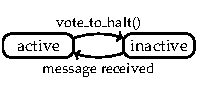
\includegraphics[width=0.35\textwidth]{figures/active.pdf}
 \caption{Vertex State Machine}
 \label{fig:voteToHalt}
\end{figure}

Besides vertex-to-vertex message passing, Pregel provides \emph{aggregators}, a mechanism for global communication.
Every vertex can provide a value to an aggregator in a superstep; the system then combines these values by a reduction operator and makes the result available at the beginning of the next superstep.
Pregel has a bunch of predefined aggregators for various types, like $\mathit{max}$ and $\mathit{min}$ for numeric values, but programmers may also define their own aggregators by providing a reduction operator and an appropriate default value.
Whether built-in or user-defined, an aggregation operator should be commutative and associative \todo{define this as ``accumulative''?}, with the default value being an identity.
Being simple, Pregel has demonstrated its usefulness in implementing many interesting graph algorithms \cite{pregel,QuWH12,connectivity,optimizing,XiYZ14}.

Google's Pregel \cite{pregel} proposed the vertex-centric computing paradigm, which allows programmers to think naturally like a vertex when designing distributed graph algorithms.
There are a bunch of open-source alternatives to the official and proprietary Pregel system, such as Apache Hama~\cite{hama}, Apache Giraph~\cite{giraph}, Catch the Wind~\cite{catchw}, GPS~\cite{gps}, GraphLab~\cite{graphlab}, PowerGraph~\cite{powergraph}, Mizan~\cite{mizan} and Pregel+\cite{pregelplus}.

\section{Problem in Existing Pregel Frameworks}

Despite the power of Pregel, it is a big challenge to implement a graph algorithm correctly and efficiently in Pregel \cite{connectivity}, especially when the algorithm consists of multiple stages and complicated data dependencies.
The main reason for this is the big gap between graph algorithms and their actual implementations:

\begin{itemize}\setlength\itemsep{0em}
\item
 \textit{Exceedingly complicated loop body}.
 A Pregel program is essentially a loop with a possibly big and complicated loop body defined by the \emph{compute()} function.
 In contrast, many typical distributed graph algorithms can be seen as the combination (composition) of smaller computation components, each being a simpler graph transformation.
\item
 \textit{Non-declarative message passing style}.
 In Pregel, each superstep processes the messages sent by other vertex in the previous superstep.
 This makes a Pregel program hard to understand, because one has to trace where the messages are from and what information they carry.
 In contrast, it is more natural to describe computation with \emph{remote data access} --- reading or writing attributes of other vertices through references --- instead of lower-level message passing.
\end{itemize}

In addition to the difficulties in mapping the graph algorithms to Pregel, the Pregel's interface is unsuitable for implementing the algorithms containing various stages or requiring data communication for different purposes, and may potentially decrease the performance.
This is due to the single message type throughout the whole computation, and the complex side effects of vertex-inactivation interface:
\begin{itemize}\setlength\itemsep{0em}
\item
 \textit{Single message type}.
 In Pregel, programmers need to specify a message type in advance, and the implement the \emph{compute()} function that handles or emits the messages in this type only.
 However, some graph algorithms actually need different message types for different purposes, in which case it may consume more space and bring the overhead of data encoding/decoding.
\item
 \textit{Side effects in vertex-inactivation}.
 Many graph algorithms can be optimized by the vertex-inactivation interface, for example to skip the vertices that are already converged.
 However, the vertex state is also used to control the termination, and affects the computation of aggregator, which makes it not always applicable in graph algorithms.
\end{itemize}

\section{Domain-Specific Languages for Pregel}

Domain-Specific Languages (DSLs) are a well-known mechanism for describing solutions in a restricted domain.
Therefore, some attempts have been made to bridge this gap by proposing domain-specific languages (DSLs), such as Green-Marl~\cite{green14}, Fregel~\cite{fregel} and s6raph~\cite{s6raph}.
On one hand, these DSLs allow programmers to write a program in a compositional way to avoid writing a big loop body, and provide neighboring data access to avoid explicit message passing.
On the other hand, the programs written in these DSLs can be automatically translated to Pregel code by fusing the components in the programs into a single loop, and mapping neighboring data access into message passing.
However, for efficient implementation, the existing DSLs impose a severe restriction on the data access, allowing data access only from neighboring vertices.
In other words, they neither permit reading data from remote vertices (other than neighboring vertices), nor support writing data in remote vertices.
This restriction makes it difficult to describe many interesting graph algorithms that need remote data access~\cite{optimizing,connectivity}.
For instance, a graph algorithm may maintain a tree structure, and let every vertex use its parent's attribute in computation.
In this case, the \textit{parent} is a reference stored on each vertex, and the expected data access is to fetch the parent's attribute through the reference.

It is, in fact, hard to equip DSLs with remote reads that has efficient implementation in Pregel.
There are two main reasons.
First, remote reads cannot be directly translated into the message passing style.
Passing messages to some vertex requires the sender to know the destination.
However, a remote read is described from the perspective of the reading vertex, which specifies (and thus knows) which remote vertex to read.
To implement the read, the remote vertex should send the data as a message to the reading vertex, but there is no guarantee that the remote vertex knows the reading vertex, so additional rounds of communication are needed to propagate information about the reading vertex to the remote vertex.
Second, remote reads would introduce more involved data dependencies, making it difficult to fuse program components into a single loop.
Things become more complicated when there is \emph{chain access}, where a remote vertex is reached by following a series of references.
It requires a more careful design of the translation (to Pregel) that has no redundant communication (i.e., only the least and sufficient data is sent when implementing data reads in Pregel).

It will be even harder to equip DSLs with not only remote reads but also remote writes.
Naively adding remote writing capabilities into these languages is dangerous, because it may produce read/write conflicts when having both remote reads and writes in the context of parallel computing.
To the best of our knowledge, the problem of translating remote reads/writes to efficient message passing in Pregel has not been well studied.  

\section{Contribution of the Thesis}

In this thesis, we tackle all the above problems by proposing a more powerful DSL called Palgol\footnote{Palgol stands for {\bf P}regel {\bf algo}rithmic {\bf l}anguage.
The system with all implementation codes and test examples is available at \url{https://bitbucket.org/zyz915/palgol}.}, which supports flexible remote data access, a more algorithmic way of representing inter-vertex communication.
%In particular, programmers are allowed to use a more declarative syntax called
%\emph{global field access}, to directly read data on remote vertices.
By structuring supersteps in a high-level vertex-centric computation model and analyzing the logic patterns of global field access, we provide a novel algorithm for compiling Palgol programs to efficient Pregel code. 
In detail, our main technical contributions are as follows:
\begin{itemize}\setlength\itemsep{0em}
\item
 We propose a new high-level model for compositional vertex-centric computation, where the concept of \emph{algorithmic supersteps} is introduced as the basic computation unit for constructing vertex-centric computation in such a way that remote reads and writes are ordered in a safe way.
 Using algorithmic supersteps along with \emph{sequence} and \emph{iteration}, graph algorithms can be expressed clearly and concisely.
\item
 Based on the new computation model, we design and implement Palgol, a more declarative and powerful DSL, which supports both remote reads and writes, and allows programmers to use a more declarative syntax called \emph{global field access} to directly read data on remote vertices.
 For efficient compilation from Palgol to Pregel, we develop a logic system to compile chain access to message passing without redundant communications, and an algorithm to translate Palgol programs to Pregel programs where the number of supersteps is reduced whenever possible.
\item
 We demonstrate the power of Palgol by working on a set of representative examples.
 Palgol is much more powerful than the existing DSLs (such as Green-Marl and Fregel); it covers all what the existing DSLs can do, and can deal with algorithms with more advanced communication patterns such as the Shiloach-Vishkin connectivity algorithm~\cite{connectivity}, where an internal tree structure needs to be maintained, and data communication is needed between parent and children.
\item
 Based on the Palgol's high-level model, we further study the efficient implementation of graph algorithms in distributed environment.
 We propose an extension of Pregel framework with message channel interfaces, which allows programmers to use different message types and separately manage or optimize each communication channel, to reduce the message size in computation.
\item
 The result of our evaluation is encouraging.
 The efficiency of Palgol is comparable with hand-written code for many representative graph algorithms on practical big graphs, where the execution time varies from $25.9\%$ speedup to $32.4\%$ slowdown and the number of supersteps can be dramatically reduced up to $51.7\%$ for complicated algorithms.
\end{itemize}

\chapter{The Palgol Language}

In this section, we present our high-level DSL Palgol to describe vertex-centric graph algorithms with flexible remote access.
We start from introducing a high-level model, in which an algorithm description has a more direct correspondence with the Pregel model.
Then we define the Palgol language based on this model, and explain its syntax and semantics.
Finally we use two examples to demonstrate how Palgol can concisely describe some Pregel algorithms using remote access.

\section{The High-Level Model}

The essence of Pregel is its vertex-centric paradigm on top of the BSP model, where programmers basically describe the local computation handling the local vertex states and incoming and outgoing messages, as described in the beginning of \autoref{sec:introduction}.
This computation model requires low-level description of message passing for implementing data communication.
%\todo{what? in most cases message passing implements data communication?}

The high-level model we will propose is to provide a bridge between an algorithm and a Pregel implementation.
On one hand, it uses remote reads and writes instead of message passing to describe vertex-centric computation, making it more suitable for describing an algorithm.
On the other hand, the model is close to the Pregel computation model, in particular using the vertex-centric paradigm and barrier synchronization, and remote reads and writes are arranged in this model to avoid data conflicts, making it possible to automatically derive a valid and efficient Pregel implementation from an algorithm description in this model.

In our high-level model, the computation is constructed from some basic components, which we call \emph{algorithmic supersteps}.
An algorithmic superstep is a piece of vertex-centric computation which takes a graph containing a set of vertices with local states
as input, and outputs the same set of vertices with new states.
Using algorithmic supersteps as basic building blocks, vertex-centric computation can be combined or repeated by two operations, \emph{sequence} and \emph{iteration}, to describe sophisticated Pregel algorithms.

\begin{figure}[t]
 \centering
 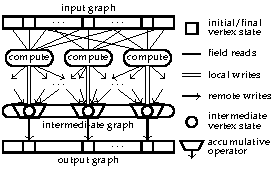
\includegraphics[width=0.75\textwidth]{figures/model.pdf}
 \caption{In an algorithmic superstep, every vertex performs local computation (including field reads and local writes) and remote updating in order.}
 \label{fig:algostep}
 \vspace{-2.5ex}
\end{figure}

The distinguishing feature of algorithmic supersteps is remote access.
Within each algorithmic superstep (illustrated in \autoref{fig:algostep}), all vertices compute in parallel, performing the same computation specified by programmers.
A vertex can read the fields of any vertex in the input graph; it can also write to arbitrary vertices to modify their fields, but the writes are performed on a separate graph rather than the input graph, to completely avoid read-write conflicts.
We further distinguish \emph{local writes} and \emph{remote writes} in our model:
local writes can only modify the current vertex's state, and are first performed on an intermediate graph (which is initially a copy of the input graph);
next, remote writes are propagated to the destination vertices to further modify their intermediate states.
Here, a remote write consists of a remote field, a value and an ``accumulative'' assignment (like \texttt{+=} and \texttt{|=}), and that field of the destination vertex is modified by executing the assignment with the value on its right-hand side.
We choose to support only accumulative assignments so that the order of performing remote writes does not matter.

More precisely, an algorithmic superstep is divided into the following two phases:
\begin{itemize}\setlength\itemsep{0em}
 \item a \emph{local computation} (LC) phase, in which a copy of the input graph is created as the intermediate graph, and then each vertex can read the state of any vertex in the input graph, perform local computation, and modify its own state in the intermediate graph, and
 \item a \emph{remote updating} (RU) phase, in which each vertex can modify the states of any vertices in the intermediate graph by sending remote writes.
After processing all remote writes are processed, the intermediate graph is returned as the output graph.
\end{itemize}
Among these two phases, the RU phase is optional, in which case the intermediate graph produced by the LC phase is used directly as the final result.

\section{An Overview of Palgol}
\label{sec:syntax}

We present our DSL Palgol next, whose design follows the high-level model we introduced in the previous subsection.
Figure~\ref{fig:syntax-simplified} shows the essential part of the syntax of Palgol.
%(A few more constructs will be introduced in Section~\ref{sec:advanced}.)
As described by the syntactic category \textit{step}, an algorithmic superstep in Palgol is a code block
enclosed by ``\textbf{for} \textit{var} \textbf{in} \textbf{V}'' and ``\textbf{end}'', where \textit{var} is a variable name that can be used in the code block for referring to the current vertex.
Such steps can then be composed (by sequencing) or iterated until a termination condition is met (by enclosing them in ``\textbf{do}'' and ``\textbf{until} \ldots'').
Palgol supports several kinds of termination conditions, but in this paper we focus on only one kind of termination condition called \textit{fixed point}, since it is extensively used in many algorithms.
The semantics of fixed-point iteration is iteratively running the program enclosed by \textbf{do} and \textbf{until}, until the specified fields stabilize.
%\todo{perhaps mention there are others}


\begin{figure}[t]
\normalsize
\[
\begin{array}{lclr}
\mathit{int} & = & \hbox{integer} \\
\mathit{float} & = & \hbox{floating-point number} \\
\mathit{var} & = & \hbox{identifier starting with lowercase letter} \\
\mathit{field} & = & \hbox{identifier starting with capital letter} \\
\\
\mathit{prog}  & \Coloneqq & \mathit{step}~|~\mathit{prog_1}\ldots\mathit{prog_n}~|~\mathit{iter} \\
\mathit{iter} & \Coloneqq & \mathbf{do}~\langle~\mathit{prog}~\rangle~\mathbf{until}~\mathbf{fix}~[~\mathit{field_1},\ldots,\mathit{field_n}~] \\
\mathit{step}& \Coloneqq & \mathbf{for}~\mathit{var}~\mathbf{in}~\mathbf{V}~\langle~\mathit{block}~\rangle~\mathbf{end} \\
\mathit{block} & \Coloneqq & \mathit{stmt_1} \ldots \mathit{stmt_n} \\
\mathit{stmt}  & \Coloneqq & \mathbf{if}~\mathit{exp}~\langle~\mathit{block}~\rangle \\
 & | & \mathbf{if}~\mathit{exp}~\langle~\mathit{block}~\rangle~\mathbf{else}~\langle~\mathit{block}~\rangle \\
 & | & \mathbf{for}~(\mathit{var}~\leftarrow~\mathit{exp})~\langle~\mathit{block}~\rangle \\
 & | & \mathbf{let}~\mathbf{mut}\mathit{_{opt}}~\mathit{var}=\mathit{exp} \\
 & | & \mathbf{local}\mathit{_{opt}}~\mathit{field}~[~\mathit{var}~]~\mathit{op_{local}}~\mathit{exp} & \hsp{-- local write} \\
 & | & \mathbf{remote}~\mathit{field}~[~\mathit{exp}~]~\mathit{op_{remote}}~\mathit{exp} & \hsp{-- remote write} \\
\mathit{exp}   & \Coloneqq & \mathit{int}~|~\mathit{float}~|~\mathit{var}~|~\mathbf{true}~|~\mathbf{false}~|~\mathbf{inf} \\
 & | & \mathbf{fst}~\mathit{exp}~|~\mathbf{snd}~\mathit{exp}~|~(\mathit{exp},\mathit{exp}) & \hsp{-- pair type} \\
 & | & \mathit{exp}.\mathbf{ref}~|~\mathit{exp}.\mathbf{val}~|~\{\mathit{exp},\mathit{exp}\} & \hsp{-- record type} \\
 & | & \mathit{exp}~?~\mathit{exp}:\mathit{exp}~|~(~\mathit{exp}~) \\
 & | & \mathit{exp}~\mathit{op_{binary}}~\mathit{exp}~|~\mathit{op_{unary}}~\mathit{exp} \\
 & | & \mathit{field}~[~\mathit{exp}~] & \hsp{-- field access} \\
 & | & \mathit{func_{opt}}~[~\mathit{exp}~|~\mathit{var}\leftarrow\mathit{exp},\mathit{exp_1},\ldots,\mathit{exp_n}~] \\
\mathit{func}  & \Coloneqq & \mathbf{maximum}~|~\mathbf{minimum} \\
 & | & \mathbf{sum}~|~\mathbf{and}~|~\mathbf{or}~|~\ldots \\
 \end{array}
\]
\caption{Essential part of Palgol syntax. Palgol is indentation-based, and two special tokens `$\langle$' and `$\rangle$' are introduced to represent the change of indentation level.}
\label{fig:syntax-simplified}
\vspace{-2ex}
\end{figure}

%As mentioned before, an algorithmic superstep has two phases, local computation (LC) and remote updating (RU).
Corresponding to an algorithmic superstep's remote access capabilities, in Palgol we can read a remote field using a field access expression of the form $\mathit{field}~[\,\mathit{exp}\,]$, and update a remote field using an accumulative assignment statement prefixed with the keyword $\mathbf{remote}$.
\begin{itemize}\setlength\itemsep{0em}
\item A field access expression $\mathit{field}~[\,\mathit{exp}\,]$, where $\mathit{exp}$ should evaluate to a vertex id, looks similar to an array access, and indeed, one can regard a field as a global array, so that when a vertex id is given, the value of the field on that vertex is returned.
\item Remote updating statements take effect only in the RU phase (after the LC phase), regardless of where they occur in the program.
Remote updating statements can only be accumulative, whereas local updating statements can be normal or accumulative assignments to the current vertex's fields.
To better distinguish the two kinds of updating statements, local updating statements can be prefixed with an optional \textbf{local} keyword.
\end{itemize}

There are some predefined fields that have special meaning in our language.
$\mathbf{Id}$ is an immutable field that stores the value of the vertex id for each vertex, whose type is user-specified but currently we can simply treat it as an integer.
$\mathbf{Nbr}$, $\mathbf{In}$, $\mathbf{Out}$ are by default the edge lists, where $\mathbf{Nbr}$ is intended to be used in undirected graphs, and $\mathbf{In}$ and $\mathbf{Out}$ respectively store incoming and outgoing edges for directed graphs.
Essentially, these are normal fields of a predefined type for representing edges, and most importantly, the compiler assumes a form of symmetry on these fields (namely that every edge is stored consistently on both of its end vertices), and uses the symmetry to produce more efficient code.

The rest of the syntax for Palgol steps is in principle similar to an ordinary programming language.
Some functional programming constructs are also used here, like let-binding and list comprehension.
To express more complicated computation, there is also a foreign function interface that allows programmers to invoke functions written in a general-purpose language.
For more details, please refer to the tutorial in our repository.

\section{A Taste of Palgol}
\label{sec:taste}

In this subsection, we use two examples to demonstrate how to describe vertex-centric algorithms in Palgol.
The first example is single-source shortest path (SSSP), and the second one is a connectivity algorithm called Shiloach-Vishkin Practical Pregel Algorithm (S-V)~\cite{connectivity}, which shows more important features of Palgol.

\subsection{Single-Source Shortest Path Algorithm}
\label{sec:sssp}

The single-source shortest path problem is among the best known in graph theory and arises in a wide variety of applications.
To understand this algorithm, we first have a look at how it is implemented in Google's Pregel system~\cite{pregel} in Figure~\ref{fig:sssp-pregel}.
\begin{figure}[thp]
\vspace{-2ex}
\begin{lstlisting}[basicstyle=\small\ttfamily,
numbers=none,language=c++,xleftmargin=0.1\textwidth]
class ShortestPathVertex : public Vertex<int, int, int> {
   void Compute(MessageIterator* msgs) {
      int minDist = vertex_id() == 0 ? 0 : INF;
      for (; !msgs->Done(); msgs->Next())
         minDist = min(minDist, msgs->Value());
      if (minDist < GetValue()) {
         *MutableValue() = minDist;
         OutEdgeIterator iter = GetOutEdgeIterator();
         for (; !iter.Done(); iter.Next())
            SendMessageTo(iter.Target(),
               minDist + iter.GetValue());
      }
      VoteToHalt();
   }
};
\end{lstlisting}
\vspace{-2ex}
\caption{Google's SSSP Pregel program~\protect\cite{pregel}}
\label{fig:sssp-pregel}
\end{figure}

This program assumes that the initial distance associated with each vertex is infinite (INF).
In each superstep, every vertex first receives messages containing the potentially minimum distances from the source computed by its neighbors, and chooses the smallest one among them.
If that distance is smaller than the one it currently stores, then it updates its own distance, and sends messages to inform all its neighbors of their potentially minimum distances from its perspective.
%, activating the neighboring vertices in the next superstep.
Every node votes to halt at the end, and in the next superstep only those nodes who have received messages will be activated.
The computation is performed iteratively until all vertices become inactive.

Despite the obscure Pregel implementation, which is cluttered with language-specific and low-level details (in particular message passing), the idea of this algorithm is fairly simple, which is an iterative computation until the following equation holds:
$$ \mathit{dist}[v] =\begin{cases}0 & \text{$v$~is the source} \\ \min_{u\in \mathit{In}(v)}~(\mathit{dist}[u]~+~\mathit{len}(v,~u)) & \text{otherwise} \end{cases} $$
We can concisely capture the essence of the shortest path algorithm in a Palgol program, as shown in Figure~\ref{fig:sssp-palgol}.
In this program, we store the distance of each vertex from the source in the $D$~field, and use a boolean field~$A$ to indicate whether the vertex is active.
There are two steps in this program.
In the first step (lines 1--4), every vertex initializes its own distance and the $A$~field.
Then comes the iterative step (lines 6--13) inside $\mathbf{do} \ldots \mathbf{until}~\mathbf{fix}~[D]$, which runs until every vertex's distance stabilizes.
Using a list comprehension (lines 7--8), each vertex iterates over all its active incoming neighbors (those whose $A$~field is true), and generates a list containing the sums of their current distances and the corresponding edge weights.
More specifically, the list comprehension goes through every edge~$e$ in the incoming edge list $\mathbf{In}\,[v]$ such that $A\,[e.\mathbf{ref}]$ is true, and puts $D\,[e.\mathbf{ref}] + e.\mathbf{val}$ in the generated list, where $e.\mathbf{ref}$ represents the neighbor's vertex id and $e.\mathbf{val}$ the edge weight.
Finally, we pick the minimum value from the generated list as \textit{minDist}, and update the local fields.

\begin{figure}[thp]
\begin{lstlisting}[basicstyle=\small\ttfamily]
for v in V
  Dist[v] := (Id[v] == 0 ? 0 : inf)
  Active[v] := (Id[v] == 0)
end
do
  for v in V
    let minDist = minimum [ Dist[e.ref] + e.val
                | e <- In[v], Active[e.ref] ]
    Active[v] := false
    if (minDist < Dist[v])
      Active[v] := true
      Dist[v] := minDist
  end
until fix[Dist]
\end{lstlisting}
\vspace{-2ex}
\caption{The SSSP program in Palgol}
\label{fig:sssp-palgol}
\end{figure}


It should be clarified that we do not intend to compile our Palgol program to the Pregel one in Figure \ref{fig:sssp-pregel}.
In fact, the Pregel code generated by the compiling algorithms in \autoref{sec:compilation} is quite different from the manually coded one.

\subsection{The Shiloach-Vishkin Connectivity Algorithm}
\label{sec:svppa}

The Shiloach-Vishkin Practical Pregel Algorithm (S-V for short)~\cite{connectivity} is a more interesting example that uses lots of important features of Palgol.
It calculates the connected components (CCs) of an undirected graph in a logarithmic 
number of supersteps.
The connectivity information is maintained using the disjoint-set data structure~\cite{disjointset}.
Specifically, the data structure is a forest, and the vertices in the same tree are regarded as belonging to the same connected component.
Each vertex maintains a parent pointer that either points to some other vertex in the same connected component, or points to itself, in which case the vertex is the root of a tree.
S-V algorithm is an iterative algorithm that begins with a forest of $n$ root nodes, and in each step it tries to discover edges connecting different trees and merge the trees together.
The description of the algorithm is shown in Figure~\ref{fig:svppa-desc}.
Readers interested in the correctness of this algorithm are referred to the original paper~\cite{connectivity} for more details.

\begin{comment}
\begin{algorithm}
\caption{Euclid's algorithm}
\label{alg:euclid}
\begin{algorithmic}[1]
\Procedure{Euclid}{$a,b$}\Comment{The g.c.d. of $a$ and $b$}
   \State $r\gets a\bmod b$
   \While{$r\not=0$}\Comment{We have the answer if $r$ is 0}
      \State $a\gets b$
      \State $b\gets r$
      \State $r\gets a\bmod b$
   \EndWhile\label{euclidendwhile}
   \State \textbf{return} $b$\Comment{The gcd is $b$}
\EndProcedure
\end{algorithmic}
\end{algorithm}

\begin{algorithm}2
 %\KwInput{an undirected graph}
 %\KwOutput{CCs represented as disjoint sets}
 %\BlankLine
 \emph{set all vertices as root nodes, i.e., every vertex initializes a pointer pointing to itself}\;
 \Repeat{the disjoint-set structure does not change}{
  \For{each vertex $u$}{
   \eIf {$u$'s parent is a root node}{
    \emph{choose a neighbor~$v$ whose parent's id is smaller than $u$'s parent's id}\;
    \emph{if $v$ exists, let $u$'s parent point to $v$'s parent}\;
   }{
    \emph{let $u$ point to its grandparent}\;
   }
  }
 }
 \BlankLine
 \vspace{-2ex}
 \caption{The S-V algorithm description}
 \label{fig:svppa-desc}
\end{algorithm}
\end{comment}

The implementation of this algorithm is complicated, which contains roughly 120 lines of code\footnote{The implementation can be accessed in \url{http://www.cse.cuhk.edu.hk/pregelplus/code/apps/basic/svplus.zip}} for the $\textit{compute()}$ function alone.
Here we just explain the message-passing-based Pregel implementation of a small part of the algorithm, to give a sense of its complexity.
For example, in the \textbf{if} statement, $u$~needs to know whether its parent~$p$ is a root node or not, i.e., whether $p$'s pointer points to $p$~itself.
The implementation achieves this by making~$p$ send its pointer to~$u$ in a previous superstep, so that $u$~can check whether $p$'s pointer points to~$p$.
Moreover, since $p$~does not maintain a list of its children, $u$~must send its own id to~$p$ in an additional superstep before $p$~sends its pointer.
We can see that, despite the simplicity of the description at algorithm level, it has to be translated into three supersteps containing a query-reply conversation between each vertex and its parent.

\begin{figure}[thp]
\begin{lstlisting}[basicstyle=\small\ttfamily]
for u in V
  D[u] := u
  D[u] <?= minimum [ e.ref | e <- Nbr[u] ]
end
do
  for u in V
    if (D[D[u]] == D[u])
      let t = minimum [ D[e.ref] | e <- Nbr[u] ]
      if (t < D[u])
        remote D[D[u]] <?= t
    else
      local D[u] := D[D[u]]
  end
until fix[D]
\end{lstlisting}
\vspace{-2ex}
\caption{The S-V program}
\label{fig:svppa-code}
\end{figure}

In contrast, the Palgol program in Figure \ref{fig:svppa-code} looks very similar to the algorithm description.
This piece of code contains two steps, where the first one (lines 1--4) just performs a simple initialization, and the other (lines 6--13) is inside an iteration as the main computation.
We use the field~$D$ to store the pointer to the parent vertex.
Let us focus on line~7, which corresponds to the $\mathbf{if}$ statement in the algorithm description that checks whether $u$'s parent is a root.
Here we simply check $D[D[u]] \shorteqq D[u]$, i.e., whether the pointer of the parent vertex $D[D[u]]$ is equal to the parent's id $D[u]$.
This expression is completely declarative, in the sense that we only specify what data is needed and what computation we want to perform, instead of explicitly implementing the message passing scheme.
All the magic happens in our compilation algorithm, which analyzes the expression and generates the message passing code.
%The first algorithmic superstep is actually very simple, which set each vertex's $D$ field to the vertex's own id.
%In our type system, $u$ and $D$ field have a special type called \textit{vertex id} or \textbf{vid} for short, and this type is mainly used in the statements or expressions involving data communication.

The rest of the algorithm can be easily associated with the Palgol program.
If $u$'s parent is a root, we generate a list containing all neighboring vertices' parent id ($D[e.\mathbf{ref}]$), and then bind the minimum one to the variable~$t$ (lines 7--8).
Now $t$~is either \textbf{inf} if the neighbor list is empty or a vertex id; in both cases we can use it to update the parent's pointer (lines 9--10) via a remote updating statement.
One important thing is that the parent vertex ($D[u]$) may receive many remote writes from its children, where only one of the children providing the minimum $t$ can successfully perform the updating.
Here, the statement \texttt{a <?= b} is an accumulative assignment, whose meaning is the same as \texttt{a := min(a, b)}.
%\todo{typeset the operators}
Finally, for the $\mathbf{else}$ branch, we locally assign $u$'s grandparent's id to $u$'s $D$ field.

The S-V program demonstrates how programmers can naturally describe a complex Pregel algorithm in Palgol, in particular using the field access syntax and the remote updating syntax.
Later we will see how such a Palgol program can be efficiently compiled into an efficient Pregel program.

\section{Vertex Inactivation}

In some Pregel algorithms, we may want to inactivate vertices during computation.
Typical examples include some matching algorithms like randomized bipartite matching~\cite{pregel} and approximate maximum weight matching~\cite{optimizing}, where matched vertices are no longer needed in subsequent computation, and the minimum spanning forest algorithm~\cite{optimizing} where the graph gradually shrinks during computation.

In Palgol, we model the behavior of inactivating vertices as a special Palgol step, which can be freely composed with other Palgol programs.
The syntactic category of \textit{step} is now defined as follows:
\[
\begin{array}{lcl}
\mathit{step} & \Coloneqq & \mathbf{for}~\mathit{var}~\mathbf{in}~\mathbf{V}~\langle~\mathit{block}~\rangle~\mathbf{end} \\
 & | & \mathbf{stop}~\mathit{var}~\mathbf{where}~\mathit{exp} \\
\end{array}
\]
The special Palgol step stops those vertices satisfying the condition specified by the boolean-valued expression \textit{exp}, which can refer to the current vertex $\mathit{var}$.
The semantics of stopping vertices is different from Pregel's voting to halt mechanism.
In Pregel, an inactive vertex can be activated by receiving messages, but such semantics is unsuitable for Palgol, since we already hide message passing from programmers.
Instead, a stopped vertex in Palgol will become immutable and never perform any subsequent local computation, but other vertices can still access its fields.
This feature is still experimental and we do not further discuss it in this paper; it is, however, essential for achieving the performance reported in \autoref{sec:evaluation}.

\section{Related Work}

To ease Pregel programming, many DSLs have been proposed, such as Palovca~\cite{palovca}, Green-Marl~\cite{green14}, Fregel~\cite{fregel} and s6raph~\cite{s6raph}.
We briefly introduce each of them below.

Palovca~\cite{palovca} is an embedded DSL using Haskell as the underlying host language for Pregel algorithms.
It expresses the Pregel APIs in Haskell using a monad, and a vertex-centric program is written in a low-level way like in typical Pregel systems.
Since this language is still low-level, programmers are faced with the same challenges in Pregel programming~\cite{green14, fregel}, mainly having to tackle all low-level details.

Green-Marl~\cite{green12} is a DSL that allows programmers to describe a graph algorithm at a higher level.
Originally proposed for graph processing on shared-memory multi-processors, it is extended~\cite{green14} to support Pregel systems, where the compilation to Pregel relies on discovering ``Pregel-canonical'' patterns.
Since it does not have a Pregel-specific language design, programmers may easily get compilation errors if they are not familiar with the implementation of the compiler.
Besides, there is still a wide range of Pregel algorithms that cannot be implemented or efficiently expressed in Green-Marl (detailed discussion is in \autoref{sec:expressiveness}), due to the limitation in expressing remote access.

Fregel~\cite{fregel} is a functional DSL for declarative programming on big graphs.
In Fregel, a vertex-centric computation is represented by a pure function that takes a graph as input and produces a new vertex state; such functions can then be composed using a set of predefined combinators to implement a complete graph algorithm.
This approach not only prevents programmers from writing invalid programs, but also helps people to better understand the behavior of a vertex-centric program.
However, due to the same reason as Green-Marl, it is also limited in expressiveness.
Moreover, when implementing the same graph algorithm, the execution time of Fregel is around an order of magnitude slower than human written code~\cite{fregel}, which makes it unsuitable for practice use.

S6raph~\cite{s6raph} is a special graph processing framework with a functional interface. It models a particular type of iterative vertex-centric computation by six functions, which are specified by programmers to implement different algorithms.
Compared to Green-Marl and Fregel, s6raph can only represent graph algorithms that contain a single iterative computing (such as PageRank and Shortest Path), while many practical Pregel algorithms are far more complicated.
In exchange, s6raph programs can be written concisely and executed efficiently.

\chapter{Compiling Palgol to Pregel}
\label{sec:compilation}

In this section, we present the compiling algorithm to transform Palgol to Pregel.
The task overall is complicated and highly technical, but the main problems are the following two: how to translate Palgol steps into Pregel supersteps, and how to implement sequence and iteration, which will be presented in \autoref{sec:trans-step} and \autoref{sec:trans-iter} respectively.
When compiling a single Palgol step, the most challenging part is the remote reads, for which we first give a detailed explanation in \autoref{sec:trans-read}.
We also mention an optimization based on Pregel's combiners in \autoref{sec:combiner}.

\section{Compiling Remote Reads}
\label{sec:trans-read}

In current Palgol, our compiler recognizes two forms of remote reads.
The first one is called \emph{consecutive field access} (or \emph{chain access} for short), which uses nested field access expressions to acquire remote data.
The second one is called \emph{neighborhood communication} where a vertex may use chain access to acquire data from \emph{all} its neighbors.
The combination of these two remote read patterns is sufficient to express quite a wide range of practical Pregel algorithms according to our experience (see the discussion in \autoref{sec:real-algos}).
In this section, we present the key algorithms to compile these two remote read patterns to message passing in Pregel.

\subsection{Consecutive Field Access Expressions}
\label{sec:consecutive}

\textbf{Definition and challenge of compiling}:
Let us begin from the first case of remote reads, which is consecutive field access expressions (or chain access) starting from the current vertex.
As an example, supposing that the current vertex is~$u$, and $D$~is a field for storing a vertex id, then $D[D[u]]$ is a consecutive field access expression, and so is $D[D[D[D[u]]]]$ (which we abbreviate to $D^4[u]$ in the rest of this section).
Generally speaking, there is no limitation on the depth of a chain access or the number of fields involved in the chain access.

As a simple example of the compilation, to evaluate $D[D[u]]$ on every vertex~$u$, a straightforward scheme is a request-reply conversation which takes two rounds of communication:
in the first superstep, every vertex~$u$ sends a request to (the vertex whose id is) $D[u]$ and the request message should contain $u$'s own id;
then in the second superstep, those vertices receiving the requests should extract the sender's ids from the messages, and reply its $D$ field to them.

When the depth of such chain access increases, it is no longer trivial to find an efficient scheme, where efficiency is measured in terms of the number of supersteps taken.
For example, to evaluate $D^4[u]$ on every vertex $u$, a simple query-reply method takes six rounds of communication by evaluating $D^2[u]$, $D^3[u]$ and $D^4[u]$ in turn, each taking two rounds, but the evaluation can actually be done in only three rounds with our compilation algorithm, which is not based on request-reply conversations.
%To this problem, we build a novel transformation algorithm, in which such scheme is easy to obtain.

\textbf{Logic system for compiling chain access}:
The key insight leading to our compilation algorithm is that we should consider not only the expression to evaluate but also the vertex on which the expression is evaluated.
To use a slightly more formal notation (inspired by Halpern and Moses~\cite{Halpern-common-knowledge}), we write $\forall u.\,\knows{v(u)}{e(u)}$, where $v(u)$~and~$e(u)$ are chain access expressions starting from~$u$, to describe the state where every vertex $v(u)$ ``knows'' the value of the expression $e(u)$; then the goal of the evaluation of $D^4[u]$ can be described as $\forall u.\,\knows{u}{D^4[u]}$.
%which means that we want to finally achieve the state that every vertex $u$ knows the result of $D^4[u]$.
Having introduced the notation, the problem can now be treated from a logical perspective, where we aim to search for a derivation of a target proposition from a few axioms.

There are three axioms in our logic system:
\begin{enumerate}
\item $\forall u.\,\knows{u}{u}$
\item $\forall u.\,\knows{u}{\mathit{D}[u]}$
\item $(\forall u.\,\knows{w(u)}{e(u)}) \wedge (\forall u.\,\knows{w(u)}{v(u)}) \implies \forall u.\,\knows{v(u)}{e(u)}$
\end{enumerate}
The first axiom says that every vertex knows its own id, and the second axiom says every vertex can directly access its local field $D$.
The third axiom encodes message passing: if we want every vertex $v(u)$ to know the value of the expression $e(u)$, then it suffices to find an intermediate vertex $w(u)$ which knows both the value of $e(u)$ and the id of $v(u)$, and thus can send the value to $v(u)$.
As an example, Figure~\ref{fig:d4u-rules} shows the solution generated by our algorithm to solve $\forall u.\,\knows{u}{D^4[u]}$, where each line is an instance of the message passing axiom.

\autoref{fig:d4u-msg} is a direct interpretation of the implications in \autoref{fig:d4u-rules}.
To reach $\forall u.\,\knows{u}{D^4[u]}$, only three rounds of communication are needed.
Each solid arrow represents an invocation of the message passing axiom in Figure~\ref{fig:d4u-rules}, and the dashed arrows represent two logical inferences, one from $\forall u.\,\knows{u}{D[u]}$ to $\forall u.\,\knows{D[u]}{D^2[u]}$ and the other from $\forall u.\,\knows{u}{D^2[u]}$ to $\forall u.\,\knows{D^2[u]}{D^4[u]}$.

\begin{figure}[t]
 \centering
 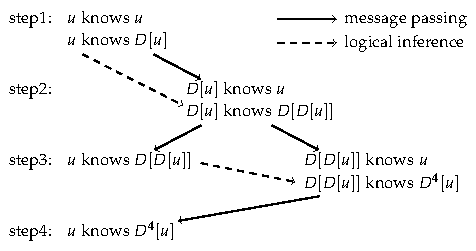
\includegraphics[width=0.75\textwidth]{figures/d4u.pdf}
 \caption{Interpretation of the derivation of $\forall u.\,\knows{u}{D^4[u]}$}
 \label{fig:d4u-msg}
\vspace{-2ex}\end{figure}

The derivation of $\forall u.\,\knows{u}{D^4[u]}$ is not unique, and there are derivations that correspond to inefficient solutions --- for example, there is also a derivation for the six-round solution based on request-reply conversations.
However, when searching for derivations, our algorithm will minimize the number of rounds of communication, as explained below.

\textbf{The compiling algorithm}:
The algorithm starts from a proposition $\forall u.\,\knows{v(u)}{e(u)}$.
%Later we will show that only considering these two patterns is enough.
The key problem here is to choose a proper $w(u)$ so that, by applying the message passing axiom backwards, we can get two potentially simpler new target propositions $\forall u.\,\knows{w(u)}{e(u)}$ and $\forall u.\,\knows{w(u)}{v(u)}$ and solve them respectively.
The range of such choices is in general unbounded, but our algorithm considers only those simpler than $v(u)$ or $e(u)$.
More formally, we say that $a$~is a \emph{subpattern} of~$b$, written $a \preceq b$, exactly when $b$~is a consecutive field access expression starting from~$a$.
%i.e., $b = \vec C[a]$ for a (possibly empty) chain $\vec C$ of fields.
For example, $u$~and $D[u]$ are subpatterns of $D[D[u]]$, while they are all subpatterns of $D^3[u]$.
The range of intermediate vertices we consider is then $\mathrm{Sub}(e(u), v(u))$, where $\mathrm{Sub}$ is defined by
\[ \mathrm{Sub}(a, b) = \{\,c \mid c \preceq a \mathrel\text{or} c \prec b \,\} \]
We can further simplify the new target propositions with the following function before solving them:
\[
\mathit{generalize}(\forall u.\,\knows{a(u)}{b(u)}) =
\begin{cases}
\forall u.\,\knows{u}{(b(u)/a(u))} & \text{if~} a(u) \preceq b(u) \\
\forall u.\,\knows{a(u)}{b(u)} & \text{otherwise}
\end{cases}
\]
where $b(u)/a(u)$ denotes the result of replacing the innermost $a(u)$ in $b(u)$ with~$u$.
(For example, $A[B[C[u]]]/C[u] = A[B[u]]$.)
This is justified because the original proposition can be instantiated from the new proposition.
(For example, $\forall u.\,\knows{C[u]}{A[B[C[u]]]}$ can be instantiated from $\forall u.\,\knows{u}{A[B[u]]}$.)

It is now possible to find an optimal solution with respect to the following inductively defined function $\mathit{step}$, which calculates the number of rounds of communication for a proposition:
\[ \setlength{\arraycolsep}{.2em}
\begin{array}{lcl}
\mathit{step}(\forall u.\,\knows{u}{u}) &=& 0 \\
\mathit{step}(\forall u.\,\knows{u}{\mathit{D}[u]}) &=& 0 \\
\mathit{step}(\forall u.\,\knows{v(u)}{e(u)}) &=& \displaystyle 1+ \min_{w(u)\in \mathrm{Sub}(e(u),v(u))}~\max(x, y) \\
\multicolumn{3}{l}{\quad\text{where}~x = \mathit{step}(\mathit{generalize}(\forall u.\,\knows{w(u)}{e(u)}))} \\
\multicolumn{3}{l}{\quad\phantom{\text{where}}~y = \mathit{step}(\mathit{generalize}(\forall u.\,\knows{w(u)}{v(u)}))}
\end{array} \]
It is straightforward to see that this is an optimization problem with optimal and overlapping substructure, which we can solve efficiently with memoization techniques.

With this powerful compiling algorithm, we are now able to handle any chain access expressions.
Furthermore, this algorithm optimizes the generated Pregel program in two aspects.
First, this algorithm derives a message passing scheme with a minimum number of supersteps, thus reduces unnecessary cost for launching supersteps in Pregel framework.
Second, by extending the memoization technique, we can ensure that a chain access expression will be evaluated exactly once even if it appears multiple times in a Palgol step, avoiding redundant message passing for the same value.


\subsection{Neighborhood Communication}
\label{sec:neighboring-access}

Neighborhood communication is another important communication pattern widely used in Pregel algorithms.
Precisely speaking, neighborhood communication refers to those chain access expressions inside a non-nested loop traversing an edge list (\textbf{Nbr}, \textbf{In} or \textbf{Out}), where the chain access expressions start from the neighboring vertex.
The following code is a typical example of neighborhood communication, which is a list comprehension used in the S-V algorithm program (Figure~\ref{fig:svppa-code}):
\begin{lstlisting}[basicstyle=\small\ttfamily,firstnumber=7]
    let t = minimum [ D[e.ref] | e <- Nbr[v] ]
\end{lstlisting}
Syntactically, a field access expression $D[e.\mathbf{ref}]$ can be easily identified as a neighborhood communication.

The compilation of such data access pattern is based on the symmetry that if \emph{all} vertices need to fetch the same field of their neighbors, that will be equivalent to making all vertices send the field to all their neighbors.
This is a well-known technique that is also adopted by Green-Marl and Fregel, so we do not go into the details and simply summarize the compilation procedure as follows:
\begin{enumerate}
 \item In the first superstep, we prepare the data from neighbors' perspective.
  Field access expressions like $D[e.\mathbf{ref}]$ now become neighboring vertices' local fields $D[u]$.
  Every vertex then sends messages containing those values to all its neighboring vertices.
 \item In the next step, every vertex scans the message list to obtain all the values of neighborhood communication, and then executes the loop according to the Palgol program.
\end{enumerate}

\section{Compiling Palgol Steps}
\label{sec:trans-step}

\begin{figure}
 \centering
 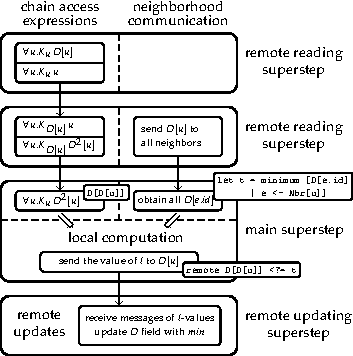
\includegraphics[width=0.75\textwidth]{figures/compile.pdf}
 \caption{Compiling a Palgol step to Pregel supersteps.}
 \label{fig:compiling-Palgol-step}
\vspace{-2ex}\end{figure}

Having introduced the compiling algorithm for remote data reads in Palgol, here we give a general picture of the compilation for a single Palgol step, as shown in \autoref{fig:compiling-Palgol-step}.
The computational content of every Palgol step is compiled into a \emph{main superstep}.
Depending on whether there are remote reads and writes, there may be a number of \emph{remote reading supersteps} before the main superstep, and a \emph{remote updating superstep} after the main superstep.

We will use the main computation step of the S-V algorithm program (lines 5--13 in \autoref{fig:svppa-code}) as a running example for explaining the compilation algorithm, which consists of the following four steps:

\begin{enumerate}
\item We first handle neighborhood communications (for S-V algorithm, $D[e.\mathbf{ref}]$ at line~7).
As mentioned at the end of \autoref{sec:neighboring-access}, the evaluation of such expressions requires a sending superstep that provides all the remote data for the loops from the neighbors' perspective (for S-V algorithm, sending their $D$~field to all their neighbors).
This sending superstep is inserted as a remote reading superstep immediately before the main superstep.

\item We analyze the chain access expressions appearing in the Palgol step with the algorithm in \autoref{sec:consecutive}, and corresponding remote reading supersteps are inserted in the front.
(For S-V algorithm, the only interesting chain access expression is $D[D[u]]$, which induces two remote reading supersteps realizing a request-reply conversation.)
In addition, our handling of neighborhood communication may introduce more chain accesses in the sending superstep, and message passing schemes should also be generated for those accesses.
(For S-V algorithm, the chain access introduced by neighborhood communication is $D[u]$, which happens to be trivial.)

\item Having handled all remote reads, the main superstep receives all the values needed and proceeds with the local computation.
Since the local computational content of a Palgol step is similar to an ordinary programming language, the transformation is straightforward except for the handling of local writes.
In general, we need to create a separate copy of all the involved fields at the beginning of the superstep.
Then, during the superstep, all field reads are performed on the original fields, and all updates are on the copies.
Finally, we use the (possibly updated) values of the copies to update the original fields at the end of the superstep.

\item What remains to be handled is the remote updating statements, which require sending the updating values as messages to the target vertices in the main superstep.
(For S-V algorithm, there is one remote updating statement at line 10, requiring that the value of~$t$ be sent to $D[u]$.)
Then an additional remote updating superstep is added after the main superstep; this additional superstep reads these messages and updates each field using the corresponding remote updating operator.
(For S-V algorithm, the minimum of all the $t$-values received is assigned to field~$D$.)

\end{enumerate}

\section{Compiling Sequences and Iterations}
\label{sec:trans-iter}

We finally tackle the problem of compiling sequence and iteration, to assemble Palgol steps into larger programs.

A Pregel program generated from Palgol code is essentially a \emph{state transition machine} (STM) combined with computation code for each state.
In the simplest case, every Palgol step is translated into a ``linear'' STM consisting of a chain of states corresponding to the supersteps like those shown in \autoref{fig:compiling-Palgol-step}.
In general, a generated STM may be depicted as:
\begin{figure}[h]
 \centering
 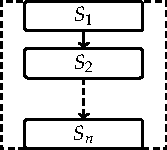
\includegraphics[width=0.25\textwidth]{figures/stm-general.pdf}
\end{figure}\\
where there are a start state and an end state, between which there can be more states and transitions, not necessarily having the linear structure.

\subsection{Compiling Sequences with STM Merging}

A sequence of two Palgol programs uses the first program to transform an initial graph to an intermediate one, which is then transformed to a final graph using the second program.
To compile the sequence, we first compile the two component programs into STMs; a composite STM is then built from these two STMs, implementing the sequence semantics.

\begin{figure}[t]
 \centering
 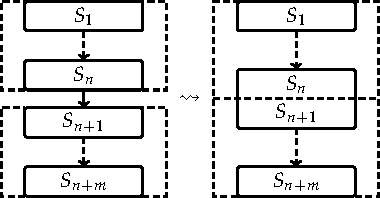
\includegraphics[width=0.6\textwidth]{figures/stm-seq.pdf}
 \caption{The compilation of sequence. A most straightforward way is shown on the left, and our compiler merges the states $S_n$ and $S_{n+1}$ and creates the STM on the right.}
 \label{fig:sequence}
\vspace{-2ex}\end{figure}

We illustrate the compilation in \autoref{fig:sequence}.
The left side is a straightforward way of compiling, and the right side is an optimized one produced by our compiler, with states $S_n$ and $S_{n+1}$ merged together.
This is because the separation of $S_n$ and $S_{n+1}$ is unnecessary:
every Palgol program describes an independent vertex-centric computation that does not rely on any incoming messages (according to our high-level model); correspondingly, our compilation ensures that the first superstep in the compiled program ignores the incoming messages.
We call this the \emph{message-independence} property.
Since $S_{n+1}$ is the beginning of the second Palgol program, it ignores the incoming messages, and therefore the barrier synchronization between $S_n$ and $S_{n+1}$ can be omitted.

\subsection{Compiling Iterations with STM Fusion}

Fixed-point iteration repeatedly runs a program enclosed by `\textbf{do}' and `\textbf{until} \ldots' until the specified fields stabilize.
To compile an iteration, we first compile its body into an STM, then we extend this STM to implement the fixed-point semantics.
The output STM is presented in \autoref{fig:fusion}, where the left one is generated by our general approach, and the right one performs the \emph{fusion optimization} when some condition is satisfied.

\begin{figure}[h]
 \centering
 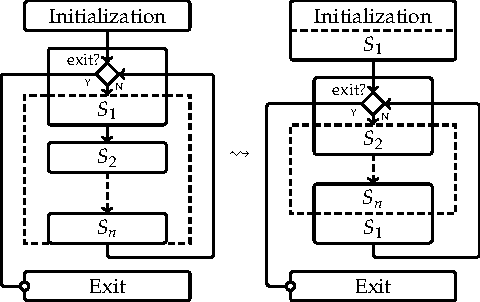
\includegraphics[width=0.75\textwidth]{figures/stm-opt.pdf}
 \caption{An STM for general iteration is shown on the left. The fusion optimization applies when the iteration body begins with a remote reading superstep ($S_1$), and yields the STM on the right.}
 \label{fig:fusion}
\vspace{-2ex}\end{figure}

Let us start from the general approach on the left.
Temporarily ignoring the initialization state, the STM implements a while loop:
first, a check of the termination condition takes place right before the state $S_1$: if the termination condition holds, we immediately enters the state \textit{Exit}; otherwise we execute the body, after which we go back to the check.
The termination check is implemented by an OR aggregator to make sure that every vertex makes the same decision:
basically, every vertex determines whether its local fields are changed during a single iteration by storing the original values before~$S_1$, and sends the result (as a boolean) to the aggregator, which can then decide globally whether there exists any vertex that has not stabilized.
What remains is the initialization state, which guarantees that the termination check will succeed in the first run, turning the while loop into a do-until loop.

There is a chance to reduce the number of supersteps in the loop body of the iteration STM when the first state $S_1$ of the loop body is a remote reading superstep (see \autoref{sec:trans-step}).
In this case, as shown on the right side of \autoref{fig:fusion}, the termination check is moved to the beginning of the second state $S_2$, and then the state $S_1$ is duplicated and attached to the end of both the initialization state and $S_n$.
This transformation ensures that, no matter from where we reach the state $S_2$, we always execute the code in $S_1$ in the previous superstep to send the necessary messages.
With this property guaranteed, we can simply iterate $S_2$ to $S_n$ to implement the iteration, so that the number of supersteps inside the iteration is reduced.
The only difference with the left STM is that we execute an extra $S_1$ attached at the end of $S_n$ when we exit the iteration.
However, it still correctly implements the semantics of iteration:
the only action performed by a remote reading superstep is sending some messages;
although unnecessary messages are emitted, the Palgol program following the extra $S_1$ will ignore all incoming messages in its first state, as dictated by the message-independence property.

\section{Combiner Optimization}
\label{sec:combiner}

Combiners are a mechanism in Pregel that may reduce the number of messages transmitted during the computation.
Essentially, in a single superstep, if all the messages sent to a vertex are only meant to be consumed by a reduce-operator (e.g., sum or maximum) to produce a value on that vertex, and the values of the individual messages are not important, then the system can combine the messages intended for the vertex into a single one by that operator, reducing the number of messages that must be transmitted and buffered.

In Pregel, combiners are not enabled by default, since ``there is no mechanical way to find a useful combining function that is consistent with the semantics of the user's \emph{compute()} method''~\cite{pregel}. %, and it is programmers' responsibility to provide an implementation for combiner.
On the other hand, Palgol's list comprehension syntax combines remote access and a reduce operator, and naturally represents such type of computation, which can potentially be optimized by a combiner.
A typical example is the SSSP program (line 7--8 in \autoref{fig:sssp-palgol}), where the distances received from the neighbors ($D[e.\mathbf{ref}]+e.\mathbf{val}$) are transmitted and reduced by the \textbf{minimum} operator.
Since the algorithm only cares about the minimum of the messages, and the compiler knows that nothing else is carried by the messages in that superstep, the compiler can automatically implement a combiner with the minimum operator to optimize the program.

\chapter{Expressiveness Analysis}
\label{sec:expressiveness}

In this chapter, we give a comprehensive comparison on the expressiveness of Palgol, Green-Marl and Fregel.
In particular, we focus on two important dimensions, the ability of representing remote access, and the ability of performing graph mutations, to give a quantitative comparison.
Finally, we review a bunch of real-world algorithms to see whether these DSLs are capable for giving an efficient implementation.

\section{Remote Access Patterns}

Palgol is able to express more remote access patterns than Green-Marl and Fregel, particularly chain access and remote writing.

Let us start from a comparison between Palgol and Fregel.
A remarkable similarity of Palgol and Fregel is that both of them use a compositional way to construct programs:
a Palgol or a Fregel program always consists of several basic units of vertex-centric computation (e.g., Palgol step, or \emph{step function} in Fregel), and put them together using combinators (e.g., sequence and iteration in Palgol, and higher-order functions in Fregel).
However, a Palgol step is more expressive than a step function, due to the following two reasons:
\begin{itemize}\setlength\itemsep{0em}
 \item a Palgol step consists of local computation and remote updating phases, whereas a step function can be thought of as only describing local computation, lacking the ability to modify other vertices' states;
 \item even when considering local computation, Palgol has highly declarative \textit{field access expressions} to express remote reads from an arbitrary vertex, but Fregel can only perform neighborhood communication (see \autoref{sec:neighboring-access}).
\end{itemize}

As for Green-Marl, this language is initially proposed for graph processing on the shared-memory model, and a ``Pregel-canonical'' subset of its programs can be compiled to Pregel.
%Green-Marl's expressiveness depends on the definition of Pregel-canonicity,
Green-Marl suffers the same problem as Fregel, where programmers cannot fetch data from an arbitrary vertex;
besides, the remote writes, according to our experience, is quite restricted and unstable in Green-Marl, which at least cannot be used inside a loop iterating over neighbor list.

The remote access abilities of the three languages are summarized in \autoref{tab:cm}.
\begin{table}[thp]
 \vspace{-2ex}
 \centering
 \caption{Comparison on Data Access Patterns}
 \label{tab:cm}
 \begin{tabular}{c|c|c|c}
  \hline
  \textbf{Data Access Pattern} & Palgol & Green-Marl & Fregel \\
  \hline\hline
  Neighborhood Reads & \cmark & \cmark & \cmark \\
  \hline
  Remote Reads & \cmark & \xmark & \xmark \\
  \hline
  Neighborhood Writes & \cmark & \xmark & \xmark \\
  \hline
  Remote Writes & \cmark & \cmark & \xmark \\
  \hline
 \end{tabular}
\vspace{-2ex}\end{table}

\section{Graph Mutation}

Some algorithms need to mutate the graph during computation.
For example, they may reverse the edges, shrink the graph, or even build an intermediate graph.
Graph mutation can also be used as optimization, for example to remove parallel edges, or delete some vertices or edges that are no longer needed.

Graph mutation is partially supported by Palgol, but has not been supported in Green-Marl or Fregel.
Both Green-Marl and Fregel consider the graph as immutable, so we cannot add or delete vertices and edges during graph processing. 
In Palgol, one can easily perform one kind of graph mutation, which is adding or removing edges from the edge lists.
Edge lists are just vertex fields named as \textit{Nbr}, \textit{In} or \textit{Out}, and they can be modified by local or remote updating statements.
However, one should make sure that the symmetry of edge lists are kept, or otherwise the generated code will work incorrectly when we further perform neighborhood communication.

There is still one limitation in Palgol (and also in Green-Marl or Fregel) that makes a small class of algorithms unable to implement, which is not having the ability to add or delete vertices.
One typical example is the algorithm for calculating bi-connected components (BCC)~\cite{connectivity}, which builds a dual graph using the edges in the original graph as the new vertices.
%We will target this problem in the future.

\begin{table}[t]
 \vspace{-2ex}
 \centering
 \caption{Comparison on Handling Graph Mutations}
 \label{tab:gm}
 \begin{tabular}{c|c|c|c}
  \hline
  \textbf{Graph Mutation Pattern} & Palgol & Green-Marl & Fregel \\
  \hline\hline
  Adding/Deleting Edges & \cmark & \xmark & \xmark \\
  \hline
  Adding/Deleting Vertices & \xmark & \xmark & \xmark \\
  \hline
 \end{tabular}
\vspace{-2ex}\end{table}

\section{Real-World Graph Algorithms}
\label{sec:real-algos}

We further compare the expressiveness of Palgol, Green-Marl and Fregel by real-world graph algorithms.
We choose a list of representative Pregel algorithms as follows:

\begin{itemize}\setlength\itemsep{0em}
 \item PageRank~\cite{pregel}
 \item Single-Source Shortest Path (SSSP)~\cite{pregel}
 \item Randomized Bipartite Matching (BM)~\cite{pregel}
 \item Shiloach-Vishkin Pregel Pregel Algorithm (S-V)~\cite{connectivity}
 \item Bi-Connected Components (BCC)~\cite{connectivity}
 \item Strongly Connected Components (SCC)~\cite{connectivity}
 \item Minimum Spanning Forest (MSF)~\cite{optimizing}
 \item Randomized Graph Coloring (GC)~\cite{optimizing}
 \item Weakly Connected Components (WCC)~\cite{optimizing}
 \item Approximate Maximum Weight Matching (MWM)~\cite{optimizing}
 \item Triangle Counting (TC)~\cite{triangle}
\end{itemize}

Except for BCC, which requires the ability of adding vertices, all the other algorithms can be implemented in Palgol.
On the other hand, many of the listed algorithms cannot be implemented in Green-Marl and Fregel, due to their limitation in remote access and graph mutation.

S-V and MSF are two algorithms that need field access from arbitrary vertex.
Both of them maintain an internal tree structure and data communication is needed between parent and children.
Such data accessing pattern is definitely not supported in Green-Marl or Fregel.
Furthermore, MSF and MWM need to modify the graph by eliminating or reconstructing edges during computation, which is also unable to be done in Green-Marl and Fregel.

The rest of the algorithms only need data fetching between neighbors, so by our understanding, Green-Marl and Fregel should be able to implement them.
However, we discover that some algorithms can be implemented more concisely and efficiently in Palgol.
For example, an important optimization in SCC and GC is that one can remove unnecessary edges during computation to reduce communication cost, which requires the ability to removing edges.

\chapter{Customizing Pregel with Message Channel Interface}
\label{sec:customized}

In this chapter, we present our customized Pregel framework with the message channel interface, which brings more opportunities of reducing messages in computation.
The customized Pregel framework is designed to be a more efficient back-end for Palgol to fully take the advantages of Palgol's high-level semantics in program optimization, but it can also serve as an extended programming model for programmers to implement graph algorithms.
By introducing the message channels, our customized Pregel framework is more convenient and efficient to handle complex communication patterns in a graph algorithm.

\section{The Message Channel Interface}

In complex graph algorithms (like S-V algorithm), a vertex may communication with different vertices in the same superstep, so that the messages for different purposes are mixed in the message list.
Although programmers can tag the messages to distinguish them, it is not an efficient solution.
Let us consider the scenario shown in \autoref{fig:multi-msg-example}.

\begin{figure}[th]
\centering
\begin{subfigure}[b]{0.45\textwidth}
 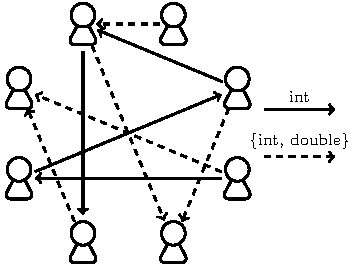
\includegraphics[width=\textwidth]{figures/multi-msg.pdf}
 \caption{space is wasted when tagging and encoding messages into the same type}
 \label{fig:multi-msg}
\end{subfigure}
\hspace{5pt}
\begin{subfigure}[b]{0.45\textwidth}
 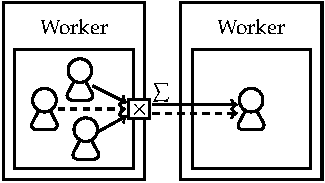
\includegraphics[width=\textwidth]{figures/comb-err.pdf}
 \caption{combiner optimization is not always applicable when different messages exist}
 \label{fig:comb-err}
\end{subfigure}
\caption{Two major problems when different messages are used in the same superstep}
\label{fig:multi-msg-example}
\end{figure}

There are two types of messages send in the same superstep, as shown in \autoref{fig:multi-msg}.
One is int type indicated by the solid arrow, and the other is a pair of int and double indicated by the dashed arrow.
In the original Pregel system, the single message type should be carefully chosen to be able to carry all types of messages used in the program.
Then, in this case, it must be at least a pair of int and double to envelope the largest possible message, which however causes a double word wasted for the messages using only int.
Moreover, the combiner optimization is not always applicable when different messages exist.
As mentioned in \autoref{sec:combiner}, the combiner is applicable when the messages are only meant to be consumed by a reduce-operator,
but when having different messages in a superstep, it is usually the case that only the messages for the same purpose can be combined.
In other words, the Pregel's combiner interface always combines \emph{all} the messages sent to the same destination vertex, but what we want is to combine a portion of the messages having the same tag, while leaving the other messages unchanged or optimized by other combiners.

The idea to solve these problem is to think communication as different channels, instead of a unified message passing interface, so that the message type or the combiner for each communication channel can be individually specified.
Furthermore, with the separation of message channels, more communication patterns in graph algorithms can be easily integrated into our system, and specialized optimization can further improve the efficiency.
%Furthermore, by separating the messages for different purposes and studying the communication patterns individually, more efficient implementation of communication patterns can be easily integrated into our system.
To illustrate this, we show that the aggregator and the request-respond paradigm \cite{effective} can be regarded as special classes of message channels, and the S-V algorithm can thus benefit from such design, and be implemented concisely and efficiently in our framework.

The remaining problem is the system design to expose a reasonably simple interface for programmers to specify and use the message channels, which will be discussed in the next section.

\section{System Design \& Implementation}

In this part, we describe the details of our system design and implementation of different types of the message channels.

\subsection{System Design}

First of all, we use the term ``worker'' to represent a basic computing unit, which in general can be a machine or a thread/process in a machine, but in our system it just refers to a process.
When launching a graph processing task, multiple instances of workers are created, and each of them holds a disjoint portion of the graph (a subset of vertices along with their attributes and edge lists).
They corporate with each other to finish the task in a distributed manner.

Workers share no memory with each other, but can exchange messages with other workers in batch through the underlying communication layer, which is implemented using the Message Passing Interface (MPI).
In particular, a worker maintains $M$ outgoing buffers (where $M$ is the number of workers), one for each worker in the cluster.
When a worker sends some data to another worker, it simply appends the data in the buffer, and it is until the end of a superstep that all the contents (not just this piece of data) in the buffer are finally delivered to their designated workers.
We accomplish it by the buffer exchange, which is implemented by $M$ rounds of pairwise communication among workers, while in each round every worker carefully selects a partner and sends the contents in the corresponding buffer through MPI's message passing primitives.
After the buffer exchange, the contents are further processed by the designated worker.

In the original Pregel system, the outgoing buffers can be seen as a single message channel which only stores the data that has the user-specified message type.
To support multiple message channels with different message types, our outgoing buffers are just raw char buffers which store serialized data only, so that data with different types can be treated equally.
Besides, the message channels buffer the messages first, and in the end if each superstep, they serialize and dump their buffers to the outgoing buffers in batch to avoid the overhead of tagging the individual messages with type information in serialization.
After the buffer exchange, the contents in the buffer are deserialized by the message channels in exactly the same order as they are serialized, to correctly restore the data.

Next, we discuss the implementation of three types of message channels: direct message passing channel, aggregator channel, and request-respond channel.

\subsection{Direct Message Passing \& Combiner}

Direct message passing is a standard mechanism provided by all Pregel framework.
In some Pregel frameworks, vertices can only send direct messages to their neighbors in the input graph, but allowing message passing between any pair of vertices is critical to make several graph algorithms~\cite{connectivity, effective} converge fast.
In our framework, the interfaces of direct message passing are shown in \autoref{fig:api-msg}.

\begin{figure}[ht]
\centering
\vspace{-2ex}
\begin{lstlisting}[basicstyle=\small\ttfamily,
numbers=none,language=c++,xleftmargin=0.1\textwidth]
template<typename VertexT, typename MsgT>
class V2V : public Serializable {
public:
   typedef typename VertexT::KeyT KeyT;
   typedef typename VertexT::HashT HashT;
   typedef void (*CombinerT)(MsgT &, const MsgT &);

   V2V(Worker<VertexT> *worker, const char *name,
       CombinerT comb = nullptr);

   void add_message(KeyT dst, const MsgT &msg);
   void send();
   bool empty();
   void reset();
   vector<vector<MsgT> >& collect();
};
\end{lstlisting}
\vspace{-2ex}
\caption{The message passing APIs}
\label{fig:api-msg}
\end{figure}

The class \texttt{V2V} represents the vertex-to-vertex communication, and it takes two type arguments: the vertex class (which includes the type of vertex identifier and a hash function), and the message type.
The constructor of class \texttt{V2V} further takes a worker, a string (for printing runtime information) and an optional combiner as arguments.
Programmers can add messages to the buffer, deliver the message after a superstep, check whether message buffer is empty, reset the class, and collect the messages sent in the previous superstep.

The implementation of the direct message passing is straightforward.
Messages are tagged with the destination vertex identifier, and added to the buffer.
If the combiner is specified, the combiner optimization is performed before serialization, by sorting and grouping the messages by the destination, and combining the messages for the same destination by a binary function.

\subsection{Aggregator}

Aggregator is also a standard mechanism for all Pregel-like frameworks, although its interface slightly differs in different frameworks.
Aggregator is to represent global communications with a specified commutative and associative operator: it collects value from every active vertex, and the combine them with the operator to a final value.
Such communication pattern is especially important for making a consensus or maintaining a same global state.
The aggregator APIs are present in \autoref{fig:api-aggregator}.

\begin{figure}[ht]
\centering
\vspace{-2ex}
\begin{lstlisting}[basicstyle=\small\ttfamily,numbers=none,language=c++]
template<typename FinalT, typename LocalT, typename InputT>
class Aggregator : public Serializable {
public:
   typedef void (*LCombinerT)(LocalT &, const InputT &);
   typedef void (*FCombinerT)(FinalT &, const LocalT &);

   Aggregator(Sync *sync, LCombinerT lc, FCombinerT fc);

   void add_value(const InputT &v);
   void aggregate();
   const FinalT &result() const;

protected:
   LocalT& local();  // access the local value
   FinalT& final();  // access the final result

private:
   virtual void init_local() = 0;
   virtual void init_final() = 0;
};
\end{lstlisting}
\vspace{-2ex}
\caption{The aggregator APIs}
\label{fig:api-aggregator}
\end{figure}

The class \texttt{Aggregator} takes three type arguments: the type of input value, the type of the partial value stored on each worker, and the type of the final result.
Two combiners need to be specified by user: one local combiner is to update the local value with an input value, and a global combiner is to update the final value by the partial values from other workers.
Meanwhile, programmers should also tell the aggregator how to initialize the local partial value and the final result before aggregation.
Programmers can feed values, perform aggregation after a superstep, and read the result of the aggregator.
The last thing to mention is that, unlike some Pregel frameworks where the aggregator automatically collects the value from all active vertices, in our system, programmers need to explicitly feed the values to the aggregator, making aggregator an independent mechanism to the vertex inactivation mechanism.

The implementation of the aggregator is also straightforward.
On each worker, a local partial value is generated from the initial value, and updated by every input value using the local combiner.
Then, each worker just sends its partial value to all other workers using the outgoing buffer interface, so that after the buffer exchange, every worker will receive the partial values from all other workers.
Then, every worker uses the global combiner to reduce them to a final value, and the order of reduction is guaranteed to be the same on all workers.

\subsection{Request-Respond Paradigm}

Request-Respond Paradigm \cite{effective} is a two-phase communication pattern that represents the communication pattern of fetching a remote vertex's attributes.
Since Pregel is a system build on ``message pushing'', such communication pattern has to be decomposed to a request and response phase:
in the request phase, each vertex sends a request to a remote vertex, then in the consequent response phase, vertices will receive the requests from other vertices, and they implicitly respond a value to them.
In this communication pattern, the number of vertices that receive requests is usually much less than the number of active vertices in the graph, which gives a chance for reducing the messages.
The solution is to let the worker merge the requests to the same destination in the sending phase, and send only 1 merged request to any destination.
Consequently, any vertex will receive at most 1 request from each worker, so that it just respond to the workers instead of to individual vertices.
Finally, when the workers receive the responses (tagged with the responser's id), they dispatch the values to the requesting vertices.

Due to the extra information kept on the sending worker, this optimization cannot be implement by the direct message passing with combiner, thus is regarded as a special communication pattern and implemented as a set of extended interfaces in Pregel+~\cite{pregelplus}.
Similar to the message passing and aggregator interface, Pregel+'s request-respond interface is shared by the whole program and the type of response value is provided by the programmer at the beginning, therefore when multiple request-respond communications are required in the program, programmers should carefully arrange them in different supersteps, and encode them to a same type.
In contrast, in our customized Pregel framework, we just implement it as another type of message channels, so programmers can specify the request-respond channels individually, which makes the implementation very easy.
%Another remarkable difference is that, Pregel+ uses an additional communication channel for request-respond paradigm, while our system implement the request-respond channel on top of the raw char buffer, which potentially reduce the number of message exchanges among workers.
The APIs of request-respond channel are presented in \autoref{fig:api-reqresp}.

\begin{figure}[ht]
\centering
\vspace{-2ex}
\begin{lstlisting}[basicstyle=\small\ttfamily,numbers=none,language=c++]
template<typename VertexT, typename ValT>
class ReqResp : public Serializable {
public:
   typedef typename VertexT::KeyT KeyT;
   typedef typename VertexT::HashT HashT;

   ReqRes(Worker<VertexT> *worker, const char *name);

   void add_request(int index, KeyT dst);
   void request();
   void respond(const vector<ValT> &val);
   void collect(vector<ValT> &val);
   void reset();
};
\end{lstlisting}
\vspace{-2ex}
\caption{The request-respond APIs}
\label{fig:api-reqresp}
\end{figure}

The class \texttt{ReqResp} takes two type arguments: the vertex class (which includes the type of vertex identifier and a hash function), and the message type.
In the request phase, programmers can add requests to buffer by invoking the function \emph{add\_request(index, dst)}, where \emph{index} is the unique index of the requesting vertex on current worker, and \emph{dst} is the destination vertex identifier.
Here, using the index of the requester (which is exposed to programmers) can significantly improve the performance, since we can feed the responses to the requesters directly through the index, which avoids the costly table lookup in the response phase.
Next, \emph{request()} should be invoked after all requests are added, to let the system preprocess the requests and deliver them after the current superstep.
The respond function \emph{respond(val)} is then invoked in the next superstep on all workers, where \emph{val} stores the values to respond for each vertex.
Note that this mechanism is implemented in a passive way: although every vertex need to prepare a value for responding the requests, the system will only access the values from the vertices that receive requests.
Finally, after the responses are exchanged, we collect the results using the \emph{collect(val)} function, which returns an array containing the requested value for each vertex.

Here we explain the implementation of request-respond message channel in detail.
First, on each worker, we buffer all the requests, which can be seen as a list of $\langle dst,index\rangle$ where $index$ is the requester's index on this worker.
In the \emph{request()} function, we sort all the requests and extract the distinct destinations from the requests, and furthermore, for each distinct destination vertex id, we record the index of its first occurrence in the request list, so we obtain the $\langle dst_{unique},index_{req}\rangle$ pairs.
It is further split into $M$ sending lists depending on where the destination vertex locates (vertex $dst$ locates on worker $w$ where $w=hash(dst)$).
The exchange of the requests and responses are straightforward.
After the response values are received, we can get the tuples containing $\langle dst_{unique},index_{req},value\rangle$ by merging the responses with the sending lists.
Finally, using $dst_{unique}$ and $index_{req}$, we can efficiently find all the requests in the sorted request buffer that has destination $dst_{unique}$, then using the index information, we efficiently feed the $value$ to all requesting vertices.

\begin{comment}
Our implementation slightly differs from the implementation of Pregel+ in two aspects.
First, when programmers send requests in a certain superstep, Pregel+ actually performs the request and response phase consecutively, so that the programmers can get the response in the next superstep.
The reason is that, Pregel+ assumes that the requesters always want to fetch a remote vertex's attribute, so by providing a \emph{respond()} interface in class \texttt{Vertex}, vertices can respond that attributes to the requesters and Pregel+ can automate the response phase.
Instead, in our system, the request phase and respond phase happen in individual supersteps, and the response value can be generated by any user-specified computation.
\end{comment}

\section{Example: The S-V Algorithm}

Programs written for our customized Pregel are quite different from those written in Pregel.
We summarize the differences as follows:
\begin{itemize}\setlength\itemsep{0em}
\item
 First, programmers can only define the computation on every vertex in Pregel.
 In contrast, our customized Pregel framework let programmers implement the computation (the \emph{compute()} function) on each worker, and by exposing the vertices stored on each worker to the programmers, they are actually programming in the vertex-centric paradigm.
\item
 Second, in Pregel systems, message passing and aggregator are two hard-coded mechanisms, and more importantly, they are shared by the whole program, so that programmers need to find a proper message type for all the communications, or implement an aggregator that encodes all the global communications.
 However, in our customized Pregel system, message passing and aggregator are just two communication channels with different implementation, so programmers can define various instances of different types of communication channels, and specify them individually in the same program.
\item
 Third, Pregel introduce the ``voting to halt'' mechanism for termination (and sometimes for program optimization), but we provide a completely different way for program termination which has a more clear semantics.
 In particular, the user-defined \emph{compute()} function returns a boolean value indicating the current worker's local decision of termination, and the whole computation terminates when all workers decide to stop.
\end{itemize}

As a running example, let's see how the S-V algorithm~\cite{connectivity} is implemented in our customized Pregel system.
The Palgol's high-level description is shown in \autoref{fig:svppa-code}, and according to the compilation algorithm presented in \autoref{sec:compilation}, the compilation result is shown in figure \autoref{fig:full}, which contains 4 supersteps.

\begin{figure}[th]
 \centering
 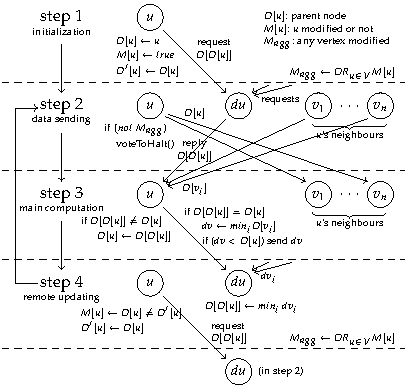
\includegraphics[width=0.8\textwidth]{figures/svppa.pdf}
 \caption{The compilation result of S-V algorithm}
 \label{fig:full}
\end{figure}

\subsection{Management of Message Channels}

Let us first consider what kind of message channels are needed for implementing the S-V algorithm.
From the compilation result of Palgol compiler, we can find three message channels, which are:
\begin{itemize}
\item
 The request-respond message channel to calculate $D[D[u]]$ in the main step.
 The request phase happens in both step 1 and step 4, while the response phase only appears in step 2.
 By following the state transition machine, we can easily verify that vertices always send the requests in the previous step of the response phase.
\item
 The direct message passing channel to collect all the neighbors' pointers to their parent, which happens between step 2 and step 3.
 The message type is the same as the type of vertex identifier.
 Note that, this message passing channel can be optimized by a combiner that calculating the minimum of the messages, since each vertex only cares about the minimum of neighbors' parent id.
\item
 The direct message passing channel to implement the remote writes in line 10 of the Palgol program shown in \autoref{fig:svppa-code}, which happens between step 3 and step 4.
 The message type is the same as the type of vertex identifier, and it can be optimized by a combiner as well, since the vertex receiving the remote writes just cares about the minimum value of the messages.
\end{itemize}

In the program, we use the variable \textit{grandpa} to represent the pointer jumping channel for calculating the grandparent (parent's parent) of every vertex, and use the variables \textit{neighbor} and \textit{remote} to represent the direct message channels for collecting all neighbors' pointer and remote writes.
The code shown in \autoref{fig:sv-declaration} defines the class \texttt{SVWorker} for implementing the S-V algorithm, declares the message channels in this class, and initializes them in the constructor.
There are three message channels defined here: two direct message channels with messages of integer message type, and one request-respond channel with integer response value.

\begin{figure}[ht]
\centering
\vspace{-2ex}
\begin{lstlisting}[basicstyle=\small\ttfamily,numbers=none,language=c++,
xleftmargin=0.1\textwidth]
typedef Vertex<int, vector<int> > VertexT;
class SVWorker : public Worker<VertexT> {
private:
   // declaration of message channels
   V2V<VertexT, int> neighbor, remote;
   ReqRes<VertexT, int> grandpa;
public:
   SVWorker():  // initialization
      grandpa(this, "Pointer Jumping"),
      neighbor(this, "Neighborhood", c_min),
      remote(this, "Remote Write", c_min) {}
   // the user-specified compute function
   bool compute() { .. }
};
\end{lstlisting}
\vspace{-2ex}
\caption{Declaration of message channels for S-V}
\label{fig:sv-declaration}
\end{figure}

%In the next section, we will show how to use these message channels in the \emph{compute()} function for data communication.

\subsection{Implementation of Individual Supersteps}

Having declared the message channels, next is to consider how to implement each superstep in the worker's \emph{compute()} function.
The \emph{compute()} function is a virtual member function of class \texttt{Worker}, and it executes different code in different superstep according to a local variable \texttt{step} to implement a multi-staged computation.
The variable \texttt{step} is guaranteed to be the same on all workers by the programmers.

\begin{figure}[ht]
\centering
\vspace{-2ex}
\begin{lstlisting}[basicstyle=\small\ttfamily,language=c++]
bool compute() {
   .. // code for other supersteps
   if (step == 3) {
      // collect messages from previous superstep
      auto &msgs = neighbor.collect();
      // collect responses from parent vertices
      grandpa.collect(D2);
      // enter vertex-centric computation
      for (int u = 0; u < numv(); u++) {
         if (D2[u] == D[u]) {
            int t = (msgs[u].empty() ? INF : 
               *min_element(msgs[u].begin(), msgs[u].end()));
            if (t < D[u])  // send an update to parent
               remote.add_message(D[u], t);
         } else
            D[u] = D2[u];
      }
      remote.send(); // deliver messages after this step
      step = 4;      // state transition
      return false;  // don't terminate
   }
   .. // code for other supersteps
}
\end{lstlisting}
\vspace{-2ex}
\caption{The implementation of step 3 for the S-V algorithm}
\label{fig:sv-step3}
\end{figure}

\autoref{fig:sv-step3} shows the implementation of the main step (step 3) for the S-V algorithm.
Before the vertex-centric computation, programmers should explicitly collect the messages form the previous superstep.
So in lines 4--7, we collect the messages from the neighbors in $msgs$ (which stores each vertex's message list) and collect the ids of grandparents in $D2$ (a list storing each vertex's grandparent).
After the messages are collected, we enter the vertex-centric computation by writing the for loop in line 9--17, in which $numv()$ is the number of vertices on the worker, $D$ is an array storing the parent vertex identifier for each vertex on this worker, and we just use the raw index to access the attributes of the vertices.
Then, since $D2$ stores the grandparent's id and $D$ stores the parent's id, the expression \texttt{D2[u] == D[u]} in line 10 checks whether a vertex's parent is a root.
If it is the case, we calculate the minimum of neighbors' parent id as $t$, and modify $u$'s parent's pointer with $t$, which is achieved by adding a message $t$ to \texttt{D[u]} by the remote updating channel $remote$.
As written in line 18, the messages buffered by the \emph{remote} channel are delivered by the function \emph{send()}, so that the messages are expected to reach the destinations in step 4, according to the state transition in line 19.
If $u$'s parent is not a root node, then current vertex $u$ modifies its pointer $D$ to $u$'s grandparent $D2[u]$ by an assignment in line 16.
Finally, in line 20, we return \texttt{false} indicating that the computation should continue after current superstep ends.

The way to implement the other supersteps are basically the same, by collecting the messages first, performing the vertex-centric computation next, and then delivering the messages, change the state, and return a proper return value.
In this example, we can see that our customized Pregel framework can naturally implement complex Pregel algorithm that have multiple message channels, and in the next chapter, we will demonstrate the efficiency of our framework, which is achieved by optimizing each message channel individually.

\begin{comment}
\subsection{Input/Output and Preprocessing} % not important in paper!!

Finally, we should pay a little bit more attention on the input/output and the preprocessing.
There is one more difference between this program and a typical Pregel program: in our program, we expose the index of each vertex to programmers, so programmers can use arrays to store the attributes of the vertices, which makes the code more clean.
\end{comment}

%\section{Related Work}



\chapter{Experimental Evaluation}
\label{sec:evaluation}

In this chapter, we are going to answer two questions: whether the programs written in Palgol is comparable to the ones written by human, and whether our customized Pregel system can compete with the original Pregel system.

\section{Evaluation of Palgol's Generated Code}

We evaluate and compare the performance of the Pregel programs generated by our Palgol compiler and manually coded Pregel programs over large real-world graphs.
The experiment is conducted on an Amazon EC2 cluster with 16 nodes (instance type is m4.large), each containing 2 vCPUs and 8G memory.

We compile Palgol code to Pregel+\footnote{http://www.cse.cuhk.edu.hk/pregelplus}, which is an open-source implementation of Pregel, though any Pregel-like system can be used.
The reason for choosing Pregel+ is that there is already a bunch of sophisticated Pregel algorithms implemented in this framework (including PageRank, SSSP, S-V algorithm, MSF and SCC), so we can get a fair comparison between our DSL and the hand-written code.
For SCC, since the manually coded Pregel program does not completely implement the algorithm and only provides an approximate solution, we are not able to compare them with our Palgol implementation.
%For MSF, the algorithm we use is a slightly different algorithm ..
Consequently, the rest three algorithms are used in the evaluation, and the experiment is conducted in Pregel+'s ordinary mode.

We use 4 real-world graph datasets in our performance evaluation, which are listed in Table~\ref{tab:datasets}:
\begin{enumerate}
\item LJ-UG\footnote{http://konect.uni-koblenz.de/networks/livejournal-groupmemberships}: a network of LiveJournal users and their group memberships;
\item Facebook\footnote{http://konect.uni-koblenz.de/networks/facebook-sg}: a friendship network of the Facebook social network;
\item LJ-DG\footnote{http://konect.uni-koblenz.de/networks/soc-LiveJournal1}: a friendship network of the LiveJournal blogging community;
\item Wikipedia\footnote{http://konect.uni-koblenz.de/networks/dbpedia-link}: the extracted hyperlink network of Wikipedia
\end{enumerate}
To evaluate those manually coded programs on these datasets, we slightly modify the code for graph loading (and data types if necessary), while the computation kernel remains the same.
For SSSP, we use a version closer to \autoref{fig:sssp-pregel}, which performs better than the one shipped with Pregel+.

\begin{table}[t]
 \centering
 \caption{Datasets for Performance Evaluation}
 \label{tab:datasets}
 \begin{tabular}{|c|c|c|c|}
  \hline
  Data & Type & $|V|$ & $|E|$ \\
  \hline\hline
  LJ-UG & undirected & 10,690,276 & 224,614,770 \\
  \hline
  Facebook & undirected & 59,216,214 & 185,044,032 \\
  \hline
  LJ-DG & directed & 4,847,571 & 68,993,773 \\
  \hline
  Wikipedia & directed & 18,268,992 & 172,183,984 \\
  \hline
 \end{tabular}
\vspace{-2ex}\end{table}

\subsection{Execution Time}

For each experiment, we measure the execution time (which consists of the computation time and communication time) and the number of supersteps of the entire execution.
All the results are averaged over 3 repeated experiments.

The runtime results of our experiments are summarized in \autoref{tab:exec}.
Each algorithm is run on the type of input graphs to which it is applicable (PR on directed graphs, for example) with 4 configurations, where the number of cores changes from 4 to 16.
As shown, the execution time of the Pregel programs generated by our Palgol compiler vary between $25.9\%$ speedup to $32.4\%$ slowdown, which is comparable with human-written ones.

Remarkably, for S-V algorithm, Palgol code takes up to $25.9\%$ less execution time compared to the manual implementation.
This is due to the efficient implementation of the fixed-point termination condition (see \autoref{sec:trans-iter}) by our Palgol compiler, while the manually coded Pregel program contains redundant communication.
For PageRank, we observed highly close execution time on the compiler-generated program and the manually implemented program, where the difference is within $1.7\%$.

The slowdown of Palgol on SSSP is mainly due to two reasons.
First, the manually coded program utilizes Pregel's voting to halt mechanism to inactivate converged vertices during computation;  this accelerates the execution since the Pregel system skips executing the \emph{compute()} function for those inactive vertices.
Second, due to the simplicity of SSSP, the manually coded program can dispense with the maintenance of a global state with an aggregator, and this further reduces the overhead.

\begin{table*}[t]
 \centering
 \caption{Comparison of Execution Time between Palgol and Manual Implementation (in seconds)}
 \label{tab:exec}
 \begin{tabular}{c|c||c|c||c|c||c|c||c|c||c}
  \hline
  \multirow{2}{*}{\textbf{Algorithm}} & \multirow{2}{*}{\textbf{Dataset}} & \multicolumn{2}{c||}{4 cores} & \multicolumn{2}{c||}{8 cores} & \multicolumn{2}{c||}{12 cores} & \multicolumn{2}{c||}{16 cores} & Comparison \\
  \cline{3-10}
  & & Palgol & Manual & Palgol & Manual & Palgol & Manual & Palgol & Manual & (Palgol to Manual) \\
  \hline\hline
  \multirow{2}{*}{S-V} & LJ-UD & 35.46 & 40.46 & 16.62 & 18.82 & 10.69 & 12.76 & 8.06 & 8.36 & $-16.2\%$ to $-3.6\%$ \\
  \cline{2-11}
  & Facebook & 146.80 & 172.33 & 84.72 & 105.50 & 65.67 & 85.70 & 56.78 & 76.61 & $-25.9\%$ to $-14.8\%$ \\
  \hline
  \multirow{2}{*}{SSSP} & LJ-DG & 3.21 & 2.98 & 1.83 & 1.78 & 1.31 & 1.23 & 0.98 & 0.93 & $2.6\%$ to $7.6\%$ \\
  \cline{2-11}
  & Wikipedia & 10.02 & 7.57 & 5.20 & 4.19 & 3.61 & 2.97 & 2.74 & 2.30 & $19.4\%$ to $32.4\%$ \\
  \hline
  \multirow{2}{*}{PR} & LJ-DG & 76.70 & 76.54 & 42.31 & 42.83 & 29.83 & 30.20 & 23.95 & 24.10 & $-1.2\%$ to $0.2\%$ \\
  \cline{2-11}
  & Wikipedia & 151.26 & 151.26 & 80.67 & 81.05 & 57.30 & 57.75 & 45.44 & 46.24 & $-1.7\%$ to $0.0\%$ \\
  \hline
 \end{tabular}
\end{table*}

\subsection{Number of Supersteps}

The number of supersteps used by the compiler-generated programs and manually coded programs are presented in \autoref{tab:steps}.
For PageRank, Palgol takes exactly the same number of supersteps as the manually coded Pregel program, and for SSSP, Palgol needs one additional superstep to terminate the program.
The reason is that Palgol needs to check whether all vertices have converged by using an aggregator, while the manual version utilizes the voting to halt mechanism, which can terminate the program immediately when all vertices have converged.

For S-V algorithm, Palgol reduces the number of supersteps by $51.7\%$.
The dramatic improvement for S-V algorithm is due to Palgol's efficient transformation of the fixed-point termination condition.
In addition, the state merging and iteration fusion optimizations can generate highly compact code.
Although such optimization is applicable to manually implemented code, it takes a lot of effort to do so especially for large programs, since state merging can easily change the whole implementation (such as message encoding, aggregator, etc).
In other words, compact programs are usually harder to maintain for humans.

\begin{table}[t]
 \centering
 \caption{Comparison of the Number of Supersteps}
 \label{tab:steps}
 \begin{tabular}{c|c|c|c|c}
  \hline
  \textbf{Algorithm} & \textbf{Dataset} & Palgol & Manual & Comparison \\
  \hline\hline
  \multirow{2}{*}{S-V} & LJ-UG & 14 & 29 & $-51.7$\% \\
  \cline{2-5}
  & Facebook & 23 & 43 & $-46.5$\% \\
  \hline
  \multirow{2}{*}{SSSP} & LJ-DG & 17 & 16 & $6.2$\% \\
  \cline{2-5}
  & Wikipedia & 50 & 49 & 2.0\% \\
  \hline
  \multirow{2}{*}{PR} & LJ-DG & 32 & 32 & $0$\% \\
  \cline{2-5}
  & Wikipedia & 32 & 32 & $0$\% \\
  \hline
 \end{tabular}
\vspace{-2ex}\end{table}

\section{Evaluation of the Customized Pregel Framework}

\chapter{Conclusions}
\label{sec:conclusions}

\section{Contributions}

This thesis proposes Palgol, a high-level domain-specific language for Pregel systems with flexible remote data access, which allows people to design and implement vertex-centric graph algorithms in a more natural way.
In particular, we tackle the problem of translating remote data read to Pregel's message passing, and by recognizing and compiling two useful remote reading patterns, chain access and neighborhood communication, Palgol can express a wider range of practical Pregel algorithms than existing languages.
Furthermore, we extend the existing Pregel system with a novel message channel interface, which
Experiment results show that graph algorithms written in Palgol can be compiled to efficient Pregel programs comparable to the human written ones.

\section{Future Directions}

As for future work, on the high-level, we are going to provide a more mature solution for vertex activation or inactivation, and support more remote access patterns in Palgol.
On the aspect of system design.


% =====================================================
%  Back Matter
% =====================================================

%\backmatter


% =====================================================
%  Bibliography
% =====================================================

%\bibliographystyle{plain}
\bibliographystyle{unsrt}
\bibliography{ref}


% =====================================================
%  Appendices
% =====================================================

\begin{appendices}

%\include{Manuscript/Tips/tips}

\end{appendices}


\end{document}
